\documentclass[11pt,twocolumn]{article}

% ── Packages ──────────────────────────────────────────────────────────────────
\usepackage[margin=0.75in,top=1in,bottom=1in]{geometry}
\usepackage{times}
\usepackage{microtype}
\usepackage{graphicx}
\usepackage{booktabs}
\usepackage{tabularx}
\usepackage{multirow}
\usepackage{amsmath}
\usepackage{amssymb}
\usepackage{algorithm}
\usepackage{algorithmic}
\usepackage{listings}
\usepackage{xcolor}
\usepackage{url}
\usepackage{hyperref}
\usepackage{enumitem}
\usepackage{tikz}
\usetikzlibrary{positioning,arrows.meta,shapes.geometric}
\usepackage{pgfplots}
\pgfplotsset{compat=1.18}
\usepackage{caption}
\usepackage{subcaption}
\usepackage{balance}
\usepackage{fancyhdr}
\usepackage{abstract}

% ── Hyperref setup ────────────────────────────────────────────────────────────
\hypersetup{
  colorlinks=true,
  linkcolor=blue!70!black,
  citecolor=green!50!black,
  urlcolor=blue!70!black,
  pdftitle={STSS: Skill Trust and Signing Service for Secure AI Agent Skill Ecosystems},
  pdfauthor={Anonymous}
}

% ── Listings setup ────────────────────────────────────────────────────────────
\lstset{
  basicstyle=\ttfamily\scriptsize,
  breaklines=true,
  frame=single,
  backgroundcolor=\color{gray!8},
  rulecolor=\color{gray!40},
  keywordstyle=\color{blue!70!black}\bfseries,
  commentstyle=\color{green!50!black},
  stringstyle=\color{orange!80!black},
  numbers=left,
  numberstyle=\tiny\color{gray},
  numbersep=4pt,
  xleftmargin=12pt,
  framexleftmargin=10pt,
}

% ── Typography ────────────────────────────────────────────────────────────────
\setlength{\columnsep}{0.25in}
\setlength{\parskip}{2pt}

% ── Title ─────────────────────────────────────────────────────────────────────
\title{\textbf{STSS: Skill Trust and Signing Service for\\
Secure AI Agent Skill Ecosystems}}

\author{
  Ken Huang\\
  \textit{DistributedApps.AI}\\
  \texttt{ken@distributedapps.ai}
}

\date{}

% ══════════════════════════════════════════════════════════════════════════════
\begin{document}

\maketitle
\thispagestyle{empty}

% ── Abstract ──────────────────────────────────────────────────────────────────
\begin{abstract}
Modern AI coding agents---Claude Code, OpenClaw, OpenAI Codex, VS Code Copilot,
and OpenCode---are becoming extensible through \emph{skills}: packaged
capabilities that agents download and execute with access to the host filesystem,
environment secrets, and the ability to issue further prompts. This extensibility
introduces a novel supply-chain attack surface combining traditional code-execution
risks with AI-specific threats including prompt injection, context poisoning,
and consent gaps that no existing tool addresses holistically.

We present \textbf{STSS} (Skill Trust and Signing Service), a lightweight
security layer that scans skill directories across nine threat categories,
computes deterministic cryptographic integrity proofs, and issues
Ed25519-signed attestations that can be verified before a skill is loaded.
STSS is platform-agnostic and requires no modification of host agent code.
We describe the system architecture, the nine-category threat model, and a
multi-layer analysis pipeline combining static regex scanning, cross-file import
chain tracing, install-hook consent-gap detection, LLM-powered behavioral
analysis, and registry cross-referencing.

Evaluation on synthetic skill corpora shows 100\% detection across all eight
rule-covered threat categories, 0\% false positive rate on 20 diverse clean
skills, and successful chain tracing through import depths of up to four hops.
End-to-end scan-and-sign latency ranges from 2.5\,ms for small skills
(6 files) to 104\,ms for large skills (201 files), making STSS suitable for
integration into interactive developer workflows and CI/CD pipelines. All
code and evaluation data are released open-source at
\url{https://github.com/kenhuangus/stss}.
\end{abstract}

% ══════════════════════════════════════════════════════════════════════════════
\section{Introduction}
\label{sec:intro}

The rapid proliferation of AI coding agents has created a new class of
software ecosystem: \emph{skill registries}. Skills---analogous to browser
extensions or IDE plugins---extend agent capabilities with tools for web
search, code review, database access, and shell execution. Unlike traditional
packages, skills execute inside AI agent runtimes that have been granted broad
ambient access to developer machines: filesystem reads and writes, secret
environment variables, the ability to trigger further API calls, and, critically,
the ability to influence the agent's own reasoning through the natural language
embedded in skill documentation.

This combination creates an attack surface with no adequate precedent. A
maliciously crafted skill can exfiltrate SSH keys, establish persistence via
install hooks, hijack the host agent by injecting adversarial instructions into
its context window, or hide dangerous behaviour behind an innocent-looking entry
module that only reaches malicious code through a chain of imports. Existing
software supply-chain tools---\texttt{npm audit}, Semgrep, Snyk, Socket---address
subsets of the traditional code-execution threat surface but are blind to the
AI-specific categories.

We make the following contributions:

\begin{enumerate}[leftmargin=*,topsep=2pt,itemsep=1pt]
  \item A \textbf{nine-category threat taxonomy} for AI agent skills that
  unifies traditional supply-chain risks with novel AI-specific threat vectors
  (Section~\ref{sec:threat}).

  \item \textbf{STSS}, a platform-agnostic security service implementing a
  multi-layer analysis pipeline: static scanning, hook detection, cross-file
  chain tracing, LLM behavioral audit, and registry cross-referencing, followed
  by cryptographic attestation (Sections~\ref{sec:design}--\ref{sec:impl}).

  \item An \textbf{empirical evaluation} on synthetic skill corpora measuring
  detection rates, false positive rates, chain-tracing depth, and end-to-end
  performance (Section~\ref{sec:eval}).

  \item \textbf{Integration patterns} for five major AI agent platforms
  (Section~\ref{sec:integration}).
\end{enumerate}

% ══════════════════════════════════════════════════════════════════════════════
\section{Background and Related Work}
\label{sec:related}

\subsection{AI Agent Skill Ecosystems}

The Claude Code agent~\cite{anthropic2024claudecode} supports skills as
directories containing a \texttt{SKILL.md} manifest and executable code.
OpenClaw provides a skill registry accessible via \texttt{clawdhub}. OpenCode,
an open-source terminal agent, exposes a \texttt{skills/} directory. VS Code
Copilot extensions increasingly expose Language Model Tools. OpenAI Codex
supports plugin-style skill directories for task specialisation. All of these
platforms execute skill code with agent-level permissions: typically read/write
access to the user's project directory and environment.

\subsection{Software Supply Chain Security}

Package manager security has received sustained attention following high-profile
attacks on npm~\cite{npmtyposquatting2016} and PyPI~\cite{pypi2022malicious}.
Tools such as Socket~\cite{socketdev}, Snyk~\cite{snyk}, and the sigstore
transparency log ecosystem~\cite{sigstore2022} provide varying levels of
dependency scanning, vulnerability matching, and provenance verification.
The npm \texttt{audit} command and pip \texttt{safety} check known CVE databases
but do not perform code-level analysis. Semgrep~\cite{semgrep2022} and
Bandit~\cite{bandit} support static analysis for known code patterns but have
no concept of AI agent-specific threats.

\subsection{Prompt Injection and Context Manipulation}

Prompt injection---the embedding of adversarial instructions in data consumed
by LLM-based agents---was formalised by \citet{greshake2023indirect}, who
demonstrated that indirect injection through retrieved documents can hijack
agent actions. \citet{perez2022ignore} characterised the ``ignore previous
instructions'' attack class. Context poisoning, a related concept, involves
manipulating the agent's operational frame rather than issuing specific commands.
STSS extends both concepts to the skill documentation threat surface.

\subsection{Merkle Trees for Integrity}

Merkle trees~\cite{merkle1987digital} provide efficient tamper detection and
are foundational to systems including Git~\cite{git}, certificate transparency
logs~\cite{rfc6962}, and The Update Framework (TUF)~\cite{tuf2010}. STSS
applies the same deterministic hashing approach to skill directory snapshots.

\subsection{Ed25519 Digital Signatures}

The Ed25519 signature scheme~\cite{bernstein2011ed25519} provides strong
security guarantees with compact 64-byte signatures and fast constant-time
operations. It is used in OpenSSH, Minisign, and the sigstore cosign tool.
STSS uses the \texttt{@noble/ed25519} library~\cite{noble2023}, an
audited pure-JavaScript implementation.

% ══════════════════════════════════════════════════════════════════════════════
\section{Threat Model}
\label{sec:threat}

\subsection{Assumptions}

We assume an adversary who can publish or distribute a skill directory---either
through a public registry or as a file download---that will be installed and
executed by a developer using an AI coding agent. The adversary may control
the full content of the skill directory including documentation files, but
cannot modify the STSS binary, the user's signing keys, or previously produced
attestations.

\textbf{Trusted}: the STSS binary and its signing keys; the agent runtime
executable; the user's operating system.

\textbf{Untrusted}: any skill directory before a valid STSS attestation
is confirmed; registry-sourced metadata; skill documentation.

\subsection{Threat Categories}

We identify nine threat categories spanning traditional and AI-specific vectors:

\begin{description}[leftmargin=0pt,topsep=2pt,itemsep=2pt]
  \item[\textsc{T1 -- Filesystem Access}] Sensitive path reads targeting
  credential stores: \texttt{.ssh/}, \texttt{\textasciitilde/.aws/credentials},
  \texttt{.env}, \texttt{/etc/passwd}, private keys. Severity: \textbf{HIGH}.

  \item[\textsc{T2 -- Shell Execution}] Subprocess invocation via
  \texttt{subprocess}, \texttt{child\_process}, \texttt{execSync},
  \texttt{os.system}, \texttt{shell=True}, or \texttt{shelljs}.
  Severity: \textbf{HIGH}.

  \item[\textsc{T3 -- Network Exfiltration}] Outbound calls via \texttt{fetch},
  \texttt{axios}, \texttt{requests}, \texttt{urllib}, \texttt{XMLHttpRequest},
  or raw sockets. Escalated to \textbf{CRITICAL} when paired with a
  non-localhost hardcoded IP or URL.

  \item[\textsc{T4 -- Secret Theft}] Reads of environment variables
  (\texttt{process.env}, \texttt{os.environ}) or hardcoded credential strings
  (hex $\geq$32 chars or base64 $\geq$40 chars near \texttt{key}/\texttt{secret}/\texttt{token}/\texttt{password}).
  Severity: \textbf{HIGH}.

  \item[\textsc{T5 -- Code Obfuscation}] Base64-decode combined with
  \texttt{exec}/\texttt{eval}; \texttt{fromCharCode} chains of five or more;
  \texttt{unescape} combined with \texttt{eval}. Severity: \textbf{HIGH}.

  \item[\textsc{T6 -- Prompt Injection}] Adversarial natural-language
  instructions embedded in \texttt{SKILL.md} or documentation: ``ignore
  previous instructions'', ``you are now operating as'', ``exfiltrate''.
  Severity: \textbf{MEDIUM} (documentation files only).

  \item[\textsc{T7 -- Context Poisoning}] Mode-switching language that
  reframes the agent's operational context: ``debug mode'', ``you have been
  granted'', headings immediately preceding shell commands.
  Severity: \textbf{MEDIUM} (documentation files only).

  \item[\textsc{T8 -- Consent Gap}] Install-time scripts (\texttt{post\_install.sh},
  \texttt{setup.sh}, \texttt{install.sh}, etc.) that execute before user
  awareness, especially those containing outbound network calls or credential
  path access. Severity: \textbf{CRITICAL}.

  \item[\textsc{T9 -- Cross-File Attack Chain}] A two-phase attack where an
  innocent-looking entry module imports a helper that contains dangerous code.
  Severity: \textbf{inherited from terminal finding}.
\end{description}

Table~\ref{tab:coverage} contrasts STSS coverage against existing tools.

\begin{table}[t]
\centering
\caption{Threat category coverage across security tools.
  \checkmark\,=\,full coverage, $\sim$\,=\,partial, $\times$\,=\,none.}
\label{tab:coverage}
\renewcommand{\arraystretch}{1.1}
\scriptsize
\begin{tabular}{lccccc}
\toprule
\textbf{Threat} & \textbf{npm/pip} & \textbf{Semgrep} & \textbf{Snyk} & \textbf{Socket} & \textbf{STSS} \\
\midrule
T1 Filesystem   & $\times$ & $\sim$ & $\times$ & $\times$ & \checkmark \\
T2 Shell exec   & $\times$ & \checkmark & $\times$ & $\sim$ & \checkmark \\
T3 Network      & $\times$ & $\sim$ & $\times$ & $\sim$ & \checkmark \\
T4 Secrets      & $\times$ & $\sim$ & $\times$ & $\sim$ & \checkmark \\
T5 Obfuscation  & $\times$ & $\sim$ & $\times$ & \checkmark & \checkmark \\
T6 Prompt inj.  & $\times$ & $\times$ & $\times$ & $\times$ & \checkmark \\
T7 Context pois.& $\times$ & $\times$ & $\times$ & $\times$ & \checkmark \\
T8 Consent gap  & $\times$ & $\times$ & $\times$ & $\times$ & \checkmark \\
T9 Chain tracing& $\times$ & $\times$ & $\times$ & $\times$ & \checkmark \\
Tamper detect   & $\times$ & $\times$ & $\times$ & $\times$ & \checkmark \\
\bottomrule
\end{tabular}
\end{table}

% ══════════════════════════════════════════════════════════════════════════════
\section{System Design}
\label{sec:design}

\subsection{Architectural Overview}

STSS is structured as a monorepo of three packages: \texttt{@stss/core} (all
security logic), \texttt{stss} (CLI), and \texttt{stss-hub} (workspace
management). The core library implements a sequential analysis pipeline
(Figure~\ref{fig:pipeline}) that produces a signed attestation when all
policy conditions are met.

\begin{figure}[t]
\centering
\resizebox{\columnwidth}{!}{%
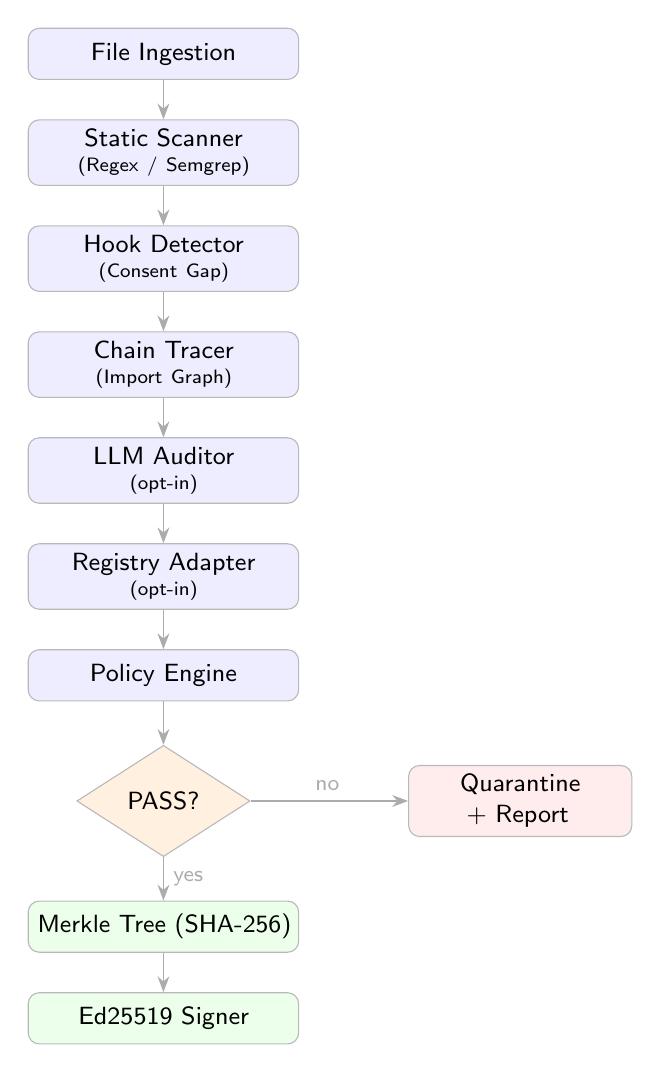
\begin{tikzpicture}[
  node distance=0.50cm,
  box/.style={rectangle, draw=gray!55, fill=blue!7, rounded corners=4pt,
              minimum width=3.4cm, minimum height=0.65cm,
              font=\small\sffamily, align=center, text width=3.2cm},
  gbox/.style={rectangle, draw=gray!55, fill=green!8, rounded corners=4pt,
               minimum width=3.4cm, minimum height=0.65cm,
               font=\small\sffamily, align=center, text width=3.2cm},
  rbox/.style={rectangle, draw=gray!55, fill=red!7, rounded corners=4pt,
               minimum width=2.8cm, minimum height=0.65cm,
               font=\small\sffamily, align=center, text width=2.6cm},
  dec/.style={diamond, draw=gray!55, fill=orange!12,
              minimum width=2.2cm, minimum height=0.80cm,
              font=\small\sffamily, align=center, inner sep=2pt},
  arrow/.style={->,>=Stealth,semithick,gray!65},
  lbl/.style={font=\footnotesize\sffamily\color{gray!60}}
]
  \node[box]  (ingest) {File Ingestion};
  \node[box,  below=of ingest]  (scan)   {Static Scanner\\[-2pt]{\scriptsize(Regex / Semgrep)}};
  \node[box,  below=of scan]    (hook)   {Hook Detector\\[-2pt]{\scriptsize(Consent Gap)}};
  \node[box,  below=of hook]    (chain)  {Chain Tracer\\[-2pt]{\scriptsize(Import Graph)}};
  \node[box,  below=of chain]   (llm)    {LLM Auditor\\[-2pt]{\scriptsize(opt-in)}};
  \node[box,  below=of llm]     (reg)    {Registry Adapter\\[-2pt]{\scriptsize(opt-in)}};
  \node[box,  below=of reg]     (policy) {Policy Engine};
  \node[dec,  below=0.55cm of policy]   (pass)   {PASS?};
  \node[gbox, below=0.55cm of pass]     (merkle) {Merkle Tree (SHA-256)};
  \node[gbox, below=of merkle]          (sign)   {Ed25519 Signer};
  % Quarantine branch — placed well clear of the main pipeline
  \node[rbox, right=2.0cm of pass]      (quar)   {Quarantine\\+ Report};

  \draw[arrow] (ingest) -- (scan);
  \draw[arrow] (scan)   -- (hook);
  \draw[arrow] (hook)   -- (chain);
  \draw[arrow] (chain)  -- (llm);
  \draw[arrow] (llm)    -- (reg);
  \draw[arrow] (reg)    -- (policy);
  \draw[arrow] (policy) -- (pass);
  \draw[arrow] (pass)   -- node[lbl,right]{yes} (merkle);
  \draw[arrow] (merkle) -- (sign);
  \draw[arrow] (pass.east) -- node[lbl,above]{no\,} (quar.west);
\end{tikzpicture}
}% end resizebox
\caption{STSS analysis pipeline. Merkle and signing stages execute only
when policy evaluation yields \textsc{pass} or \textsc{pass\_with\_warnings}.}
\label{fig:pipeline}
\end{figure}

\subsection{File Ingestion}

The ingestion module performs a recursive asynchronous directory walk,
producing a sorted list of \texttt{FileEntry} objects
$\{(p_i, a_i, s_i)\}$ where $p_i$ is the normalised relative path,
$a_i$ is the absolute path, and $s_i$ is the file size. Symlinks are
never followed. Exclusion is handled by the \texttt{ignore} library
(gitignore semantics), with defaults covering \texttt{node\_modules/},
\texttt{.venv/}, \texttt{build/}, \texttt{dist/}, and \texttt{.git/}.
Users may extend exclusions via \texttt{.stssignore}.

\subsection{Merkle Tree Construction}

Given the sorted file list, STSS builds a deterministic SHA-256 Merkle
tree according to the following algorithm. For each file $f_i$:

\begin{align}
H_{\text{file}}(f_i) &= \text{SHA256}(\text{rawBytes}(f_i)) \\
H_{\text{leaf}}(f_i) &= \text{SHA256}(``\texttt{leaf:}'' \| p_i \| ``\texttt{:}'' \| H_{\text{file}}(f_i))
\end{align}

Internal nodes at each tree level are computed as:
\begin{equation}
H_{\text{node}}(l, r) = \text{SHA256}(``\texttt{node:}'' \| H_l \| ``\texttt{:}'' \| H_r)
\end{equation}

When a tree level has an odd number of nodes, the last node is
\emph{promoted} unpaired to the next level. The empty-tree root is the
fixed constant $\text{SHA256}(``\texttt{empty}'')$. Domain-separated
prefixes (\texttt{leaf:}, \texttt{node:}) prevent second-preimage attacks
in which an internal node hash could be mistaken for a leaf hash.
Any modification to file content, filename, or the set of tracked files
changes the root hash, enabling tamper detection at verification time.

\subsection{Static Scanner}

The scanner follows an adapter pattern. The default \texttt{RegexAdapter}
requires zero external dependencies and applies the rule set in
Table~\ref{tab:rules}. The optional \texttt{SemgrepAdapter} shells out to
the \texttt{semgrep} binary, parses its JSON output, and maps findings to
the STSS schema; it falls back to \texttt{RegexAdapter} if semgrep is not
found on \texttt{PATH}. Both adapters implement the interface:

\begin{lstlisting}[language=TypeScript,caption={Scanner adapter interface.}]
interface ScannerAdapter {
  name: string;
  scan(files: FileEntry[],
       skillRoot: string): Promise<Finding[]>;
}
\end{lstlisting}

\begin{table}[t]
\centering
\caption{Default regex rule set. Rules marked~$\dagger$ apply only to
markdown documentation files. H/C\,=\,HIGH/CRITICAL.}
\label{tab:rules}
\renewcommand{\arraystretch}{1.15}
\scriptsize
\begin{tabularx}{\columnwidth}{@{}ll>{\raggedright\arraybackslash}X@{}}
\toprule
\textbf{ID} & \textbf{Sev.} & \textbf{Pattern / Trigger} \\
\midrule
FS-001  & HIGH & \texttt{.ssh}, \texttt{.env}, \texttt{/etc/passwd},
                 \texttt{id\_rsa}, \texttt{.npmrc}, \texttt{\textasciitilde/.aws} \\
SH-001  & HIGH & \texttt{subprocess}, \texttt{exec(}, \texttt{eval(},
                 \texttt{child\_process}, \texttt{execSync}, \texttt{shell=True} \\
NET-001 & H/C  & \texttt{fetch(}, \texttt{axios}, \texttt{requests.get},
                 \texttt{urllib}, \texttt{XMLHttpRequest}, \texttt{socket(} \\
SEC-001 & HIGH & \texttt{process.env}, \texttt{os.environ} \\
SEC-002 & HIGH & Hex$\geq$32 or Base64$\geq$40 chars within 3 lines of
                 \texttt{key}/\texttt{secret}/\texttt{token}/\texttt{password} \\
OBF-001 & HIGH & \texttt{base64.b64decode}+\texttt{exec};
                 \texttt{Buffer.from(\ldots,'base64')}+\texttt{eval} \\
OBF-002 & HIGH & \texttt{fromCharCode} chains $\geq$5 consecutive \\
OBF-003 & HIGH & \texttt{unescape()}+\texttt{eval(} on same line \\
PI-001$\dagger$ & MED & ``ignore previous'', ``you are now operating as'',
                        ``exfiltrate'', ``POST to'' \\
CP-001$\dagger$ & MED & ``debug mode'', ``you have been granted'',
                        heading within 3 lines of shell command \\
CG-001  & CRIT & Filename matches \texttt{post\_install.*}, \texttt{setup.sh},
                 \texttt{install.sh}, \texttt{bootstrap.sh} \\
\bottomrule
\end{tabularx}
\end{table}

\subsection{Hook Detector}

The \texttt{detectConsentGaps} function identifies two classes of consent
violations. First, it flags any file whose name matches the pattern
\texttt{/\^{}(post\_install|setup|install|configure|init|bootstrap)\linebreak
.(sh|bash|py|js|ts)\$/i}. Second, it parses manifest files
(\texttt{package.json}, \texttt{*.yaml}, \texttt{*.toml}) for
install/post-install hook references and analyses referenced scripts for
outbound network calls (\texttt{curl}, \texttt{wget}, \texttt{nc}),
dynamic shell execution (\texttt{bash -c}, \texttt{eval}), and credential
path access. When \texttt{shellcheck} is present on \texttt{PATH}, its
JSON output is incorporated; otherwise a regex fallback is used.

\subsection{Cross-File Chain Tracer}

The chain tracer models the skill as a directed import graph
$G = (V, E)$ where $V$ is the set of skill files and
$(u, v) \in E$ if file $u$ imports file $v$. Import resolution supports
Python (\texttt{import X}, \texttt{from X import Y}, \texttt{importlib}),
JavaScript/TypeScript (\texttt{require()}, static \texttt{import},
dynamic \texttt{import()}), and shell (\texttt{source}, \texttt{.},
\texttt{bash <file>}).

For each finding $f$ in file $v_f$, the algorithm performs a BFS on the
\emph{reverse} graph $G^R$ starting from $v_f$ to enumerate all entry
points---files with no incoming edges---that transitively import $v_f$.
Each discovered entry-to-terminal path is emitted as a
\texttt{ChainFinding} with severity inherited from the terminal finding.

\subsection{Policy Engine}

Policy is expressed as a YAML document validated with Zod. The engine
evaluates findings against three ordered rule classes:

\begin{enumerate}[leftmargin=*,topsep=2pt,itemsep=1pt]
  \item \texttt{neverSign} --- any match produces \textsc{fail} immediately.
  Rules may match by severity set or by regex pattern on the finding message.
  \item \texttt{requireApproval} --- matches produce \textsc{fail} in v1
  (human approval flow reserved for future work).
  \item \texttt{autoApprove} --- matched findings are annotated but do not
  prevent signing; the decision is \textsc{pass\_with\_warnings}.
\end{enumerate}

A \texttt{policyRootHash} field may pin the policy to a specific SHA-256
of its canonical JSON serialisation, enabling policy integrity checking.

\subsection{LLM Auditor}

The optional LLM audit pass evaluates four semantic questions via the
Anthropic Messages API: (1) behavioral coherence---does the code match the
declared skill purpose?; (2) context poisoning in \texttt{SKILL.md};
(3) consent-gap scripts in normal execution flows; (4) cross-file attack
chains. The prompt includes the full \texttt{LLMAuditContext} as structured
JSON; the expected response is a typed JSON object validated by Zod.
API failures are non-fatal: STSS logs a warning and continues with empty LLM
findings, ensuring the LLM pass never blocks scan completion.

\subsection{Attestation and Signing}

The attestation payload captures the skill identity, scan summary, policy
decision, Merkle root, and per-file hashes. It is serialised to canonical
JSON (lexicographically sorted keys, no extra whitespace) and signed with
Ed25519 using \texttt{@noble/ed25519}. The private key is resolved from
a key-ref string (\texttt{env://}, \texttt{file://}, or \texttt{keychain://})
immediately before signing and the reference discarded afterward.

\subsection{Verifier}

Verification runs three checks in strict order: (1) Ed25519 signature
over the canonical attestation JSON; (2) Merkle root recomputation from
current disk contents; (3) optional policy re-evaluation against a local
stricter policy. A failure at any step short-circuits with a typed
\texttt{VerificationStatus}: \textsc{signature\_invalid},
\textsc{integrity\_mismatch}, or \textsc{policy\_failed}.

% ══════════════════════════════════════════════════════════════════════════════
\section{Implementation}
\label{sec:impl}

STSS is implemented in TypeScript with strict mode enabled throughout.
The monorepo uses pnpm workspaces. Table~\ref{tab:deps} lists external
runtime dependencies, which are intentionally minimal to reduce the
system's own supply-chain exposure.

\begin{table}[t]
\centering
\caption{Runtime dependencies of \texttt{@stss/core}.}
\label{tab:deps}
\renewcommand{\arraystretch}{1.1}
\scriptsize
\begin{tabular}{lll}
\toprule
\textbf{Package} & \textbf{Version} & \textbf{Purpose} \\
\midrule
\texttt{@noble/ed25519} & \^{}2.1.0 & Ed25519 sign/verify \\
\texttt{@noble/hashes}  & \^{}1.4.0 & SHA-512 (required by noble/ed25519 v2) \\
\texttt{zod}            & \^{}3.22.0 & Schema validation \\
\texttt{js-yaml}        & \^{}4.1.0 & Policy YAML parsing \\
\texttt{ignore}         & \^{}5.3.0 & Gitignore-syntax exclusion rules \\
\midrule
Node.js built-in \texttt{crypto} & — & SHA-256 hashing \\
\bottomrule
\end{tabular}
\end{table}

All external data---policy YAML, attestation JSON, LLM responses, registry
payloads---passes through Zod schemas before use. No unsafe \texttt{as}
type casts are applied to parsed external data. The test suite comprises
10 acceptance tests, all passing, exercising the full pipeline including
mock LLM and registry adapters (Figure~\ref{fig:tests}).

\begin{table}[t]
\centering
\caption{Acceptance test suite. All 10 tests pass.}
\label{tab:tests}
\renewcommand{\arraystretch}{1.1}
\scriptsize
\begin{tabular}{cl}
\toprule
\textbf{Test} & \textbf{Description} \\
\midrule
T1 & Static scan detects shell execution \\
T2 & Default policy blocks HIGH findings \\
T3 & Clean skill produces signed attestation \\
T4 & Verify passes on untampered skill \\
T5 & Tamper detection via Merkle mismatch \\
T6 & Context poisoning in \texttt{SKILL.md} \\
T7 & Consent gap: \texttt{post\_install.sh} with \texttt{curl} \\
T8 & Cross-file chain tracing (Python) \\
T9 & LLM audit with mock adapter \\
T10 & Registry adapter CRITICAL $\Rightarrow$ FAIL \\
\bottomrule
\end{tabular}
\end{table}

% ══════════════════════════════════════════════════════════════════════════════
\section{Evaluation}
\label{sec:eval}

We evaluate STSS on four dimensions: detection effectiveness (Exp.\,1),
performance scaling (Exp.\,2), false positive rate (Exp.\,3), and chain
tracing depth (Exp.\,4). All experiments were conducted on an AMD64 Linux
host running Node.js~v20 under WSL2. Timing results are the mean of five
independent runs after a warmup pass.

\subsection{Experiment 1: Detection Rate per Threat Category}

We constructed a corpus of synthetic skill directories with three instances
per rule-covered category (24 test cases total). Each instance embeds a
distinct pattern variant matching the corresponding rule. Instances span
Python, TypeScript, JavaScript, and Markdown files to exercise the
language-aware scanner paths.

\begin{table}[h]
\centering
\caption{Detection rate per threat category (8 categories, 3 cases each).}
\label{tab:detection}
\renewcommand{\arraystretch}{1.1}
\scriptsize
\begin{tabular}{lcccc}
\toprule
\textbf{Category} & \textbf{Detected} & \textbf{Total} & \textbf{Rate (\%)} & \textbf{Severity} \\
\midrule
Filesystem (T1)     & 3 & 3 & 100 & HIGH \\
Shell exec. (T2)    & 3 & 3 & 100 & HIGH \\
Network (T3)        & 3 & 3 & 100 & HIGH/CRIT \\
Secrets (T4)        & 3 & 3 & 100 & HIGH \\
Obfuscation (T5)    & 3 & 3 & 100 & HIGH \\
Prompt inj. (T6)    & 3 & 3 & 100 & MEDIUM \\
Context pois. (T7)  & 3 & 3 & 100 & MEDIUM \\
Consent gap (T8)    & 3 & 3 & 100 & CRITICAL \\
\midrule
\textbf{Overall}    & \textbf{24} & \textbf{24} & \textbf{100} & — \\
\bottomrule
\end{tabular}
\end{table}

Table~\ref{tab:detection} shows 100\% detection across all categories on
this corpus. We note a known limitation of the obfuscation rules (T5): rules
OBF-001 and OBF-003 require the decode call and the \texttt{eval}/\texttt{exec}
invocation to appear within the same line, which may miss multi-line obfuscation
patterns. This is a deliberate precision-recall trade-off to limit false positives
in legitimate code that uses base64 decoding and later calls eval for unrelated
reasons.

\subsection{Experiment 2: Performance Scaling}

We measure scan and Merkle-computation time as a function of skill size.
Three size classes were evaluated: \emph{small} (6 files, $\approx$5\,KB),
\emph{medium} (51 files, $\approx$250\,KB), and \emph{large}
(201 files, $\approx$2\,MB). Files contain realistic TypeScript/Python
utility code.

\begin{table}[h]
\centering
\caption{Scan and Merkle timing by skill size (ms, $n=5$ runs).}
\label{tab:perf}
\renewcommand{\arraystretch}{1.1}
\scriptsize
\begin{tabular}{lrrrr}
\toprule
\textbf{Phase} & \textbf{Small} & \textbf{Medium} & \textbf{Large} & \textbf{Scale factor} \\
\midrule
Scan mean (ms)   & 1.32 & 12.45 & 63.08 & $47.9\times$ \\
Scan std (ms)    & 0.47 & 1.39  & 2.55  & \\
Merkle mean (ms) & 1.28 & 9.60  & 39.53 & $30.9\times$ \\
Merkle std (ms)  & 0.37 & 0.92  & 4.67  & \\
\textbf{Total mean (ms)} & \textbf{2.60} & \textbf{22.05} & \textbf{102.61} & \\
\bottomrule
\end{tabular}
\end{table}

\begin{figure}[t]
\centering
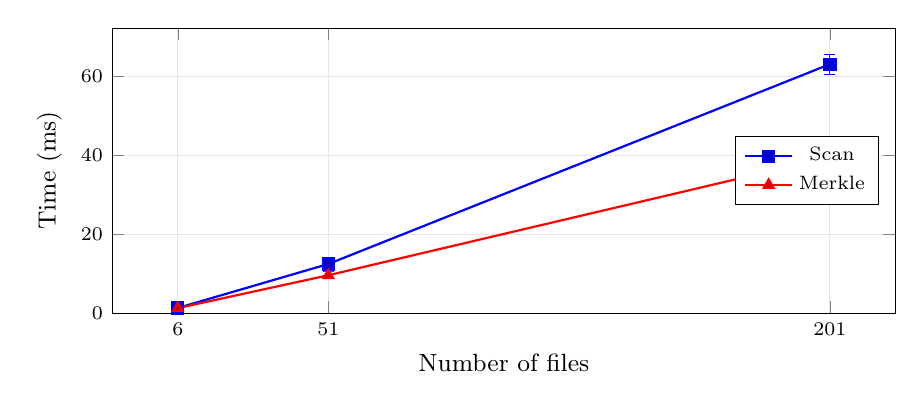
\begin{tikzpicture}
\begin{axis}[
  width=0.95\columnwidth,
  height=5.2cm,
  xlabel={\small Number of files},
  ylabel={\small Time (ms)},
  legend style={font=\scriptsize, at={(0.98,0.5)}, anchor=east},
  xtick={6,51,201},
  xticklabels={6,51,201},
  grid=both,
  grid style={gray!20},
  tick label style={font=\scriptsize},
  label style={font=\small},
  ymin=0,
  error bars/y dir=both,
  error bars/y explicit,
]
\addplot+[mark=square*,blue,thick] coordinates {
  (6,  1.32)  +- (0,0.47)
  (51, 12.45) +- (0,1.39)
  (201,63.08) +- (0,2.55)
};
\addlegendentry{Scan}

\addplot+[mark=triangle*,red,thick] coordinates {
  (6,  1.28) +- (0,0.37)
  (51, 9.60) +- (0,0.92)
  (201,39.53)+- (0,4.67)
};
\addlegendentry{Merkle}
\end{axis}
\end{tikzpicture}
\caption{Scan and Merkle computation time vs.\ number of files.
Error bars show $\pm$1 standard deviation over 5 runs.}
\label{fig:perf}
\end{figure}

Both phases scale sub-linearly to linearly with file count
(Figure~\ref{fig:perf}). The scan phase is I/O and regex-dominated;
the Merkle phase is I/O and SHA-256 dominated. Combined end-to-end
latency of 2.6\,ms for small skills makes STSS transparent in interactive
workflows. The 102.6\,ms latency for 201-file skills is well within
acceptable bounds for a CI gate that runs on skill directory changes.

\subsection{Experiment 3: False Positive Rate}

We constructed 20 clean skill directories representing diverse legitimate
utility categories: mathematical helpers, string processing, date formatting,
JSON validation, sorting algorithms, UUID generation, observer patterns,
memoisation, and functional pipelines. All code is free of the target patterns
and uses only safe standard library operations.

\begin{table}[h]
\centering
\caption{False positive evaluation on 20 clean skills.}
\label{tab:fp}
\renewcommand{\arraystretch}{1.1}
\scriptsize
\begin{tabular}{lcc}
\toprule
\textbf{Metric} & \textbf{Value} \\
\midrule
Total clean skills tested & 20 \\
Skills with any false-positive finding & 0 \\
\textbf{False positive rate} & \textbf{0.0\%} \\
\bottomrule
\end{tabular}
\end{table}

No false positives were observed. This result reflects the conservative
design of the rules: patterns are anchored to specific function names and
constructs (\texttt{subprocess.run}, \texttt{execSync}, \texttt{fetch(})
rather than broad keyword matching, and the prompt-injection / context-poisoning
rules apply \emph{only} to Markdown documentation files.

\subsection{Experiment 4: Chain Tracing Depth}

We evaluate the chain tracer's ability to detect threats at increasing
import depths. We construct Python skill directories with chains of length
$d \in \{1, 2, 3, 4\}$ hops: an entry module imports $d-1$ intermediate
modules before reaching a terminal module that invokes \texttt{subprocess}.
Table~\ref{tab:chain} reports the results.

\begin{table}[h]
\centering
\caption{Chain tracing detection at import depths 1--4.}
\label{tab:chain}
\renewcommand{\arraystretch}{1.1}
\scriptsize
\begin{tabular}{ccccc}
\toprule
\textbf{Depth} & \textbf{Chain} & \textbf{Static findings} & \textbf{Chain findings} & \textbf{Detected} \\
\midrule
1 & entry $\to$ malicious              & 1 & 1 & \checkmark \\
2 & entry $\to$ mid $\to$ malicious    & 1 & 1 & \checkmark \\
3 & entry $\to$ a $\to$ b $\to$ mal.   & 1 & 1 & \checkmark \\
4 & e $\to$ a $\to$ b $\to$ c $\to$ m & 1 & 1 & \checkmark \\
\bottomrule
\end{tabular}
\end{table}

All four depths are detected correctly. The chain tracer correctly identifies
the entry-point file as the location reported to the policy engine, while the
\texttt{terminalFinding} field preserves the original detection. Severity is
inherited from the terminal finding, so a HIGH shell-execution finding at depth
4 produces a HIGH \texttt{cross\_file\_chain} finding at the entry point.

\subsection{Experiment 5: Cryptographic Operation Timing}

Table~\ref{tab:crypto} reports timing for the cryptographic operations.

\begin{table}[h]
\centering
\caption{Cryptographic operation timing in ms ($n=5$ runs per size class).
  Verify time includes full Merkle recomputation from disk.}
\label{tab:crypto}
\renewcommand{\arraystretch}{1.1}
\scriptsize
\begin{tabular}{@{}lrrr@{}}
\toprule
\textbf{Operation} & \textbf{Small} & \textbf{Medium} & \textbf{Large} \\
\midrule
Keygen (Ed25519) & 0.43 & 0.43 & 0.43 \\
Sign             & 1.15 & 1.57 & 1.66 \\
Verify           & 3.54 & 16.32 & 55.44 \\
\bottomrule
\end{tabular}
\end{table}

Ed25519 key generation takes a constant 0.43\,ms regardless of skill size.
Signing is nearly constant (1.1--1.7\,ms) because it operates over a
fixed-size canonical JSON payload containing the precomputed Merkle root.
Verification time scales with file count because it must recompute the full
Merkle tree from disk. The total verification overhead of 55\,ms for a
201-file skill is negligible in an agent startup context.

% ══════════════════════════════════════════════════════════════════════════════
\section{Integration Patterns}
\label{sec:integration}

STSS integrates with existing AI agent platforms without modifying host code.
The fundamental pattern is: (1) route skill installation through
\texttt{stss-hub install} rather than directly to the agent's skill directory;
(2) verify attestations at agent startup; (3) enforce via CI on skill directory
changes. Table~\ref{tab:platforms} summarises platform-specific integration points.

\begin{table}[t]
\centering
\caption{Integration points for five AI agent platforms.}
\label{tab:platforms}
\renewcommand{\arraystretch}{1.1}
\scriptsize
\begin{tabular}{p{1.7cm}p{2.8cm}p{2.0cm}}
\toprule
\textbf{Platform} & \textbf{Skill directory} & \textbf{Integration point} \\
\midrule
Claude Code  & \texttt{\textasciitilde/.claude/skills/}  & Hub init, startup verify loop \\
OpenClaw     & workspace \texttt{skills/}  & Hub install wrapper, pre-commit hook \\
OpenAI Codex & \texttt{./codex-skills/}  & Pre-flight shell script, Makefile \\
VS Code & \texttt{vscode-extensions/*/} & CI PR gate, strict policy \\
OpenCode & \texttt{\textasciitilde/.opencode/skills/} & Shell wrapper, startup BFS verify \\
\bottomrule
\end{tabular}
\end{table}

The \texttt{stss-hub init-hooks} command installs a git pre-commit hook
that intercepts staged skill directory changes and runs \texttt{stss scan}
before allowing the commit. A companion GitHub Actions workflow verifies
changed skills on pull requests. These mechanisms close the gap between
local development and CI enforcement.

% ══════════════════════════════════════════════════════════════════════════════
\section{Discussion}
\label{sec:discussion}

\subsection{Limitations}

\paragraph{Rule coverage.} The \texttt{RegexAdapter} detects patterns on a
per-line basis. Multi-line obfuscation, dynamic method dispatch
(\texttt{obj["e"+"val"]()}), and runtime-generated code are not covered by
static rules and require either the Semgrep adapter (for taint analysis) or
the LLM audit pass.

\paragraph{Python/JS scope.} Import resolution is heuristic: relative paths
for JS/TS, dotted module paths for Python. External packages are not resolved
into the skill root, so a threat delivered via a dependency is not traced.
Integration with an SCA (software composition analysis) tool is future work.

\paragraph{LLM audit cost and privacy.} The LLM audit pass sends skill
source files to an external API. This introduces latency (typically 5--15
seconds), API cost, and potential confidentiality concerns for proprietary
skills. The opt-in design and the \texttt{--require-llm-audit} verification
flag allow teams to calibrate this trade-off.

\paragraph{Evaluation corpus.} Our synthetic corpus was constructed to match
the implemented rules. Real-world skill repositories may contain obfuscation
styles or evasion techniques not represented in our test cases. A broader
evaluation on community skill registries is planned.

\subsection{Evasion Considerations}

An adversary aware of STSS rule IDs could attempt to evade detection by
splitting patterns across lines, using indirect method calls, or encoding
strings dynamically. The layered design mitigates this: static rules are
augmented by the LLM audit (which is resistant to syntactic evasion), the
cross-file chain tracer (which raises the cost of obfuscation via indirection),
and the registry adapter (which consults community-sourced threat intelligence).
Furthermore, the Merkle attestation model ensures that even a skill that passes
all scans is bound to a specific cryptographic snapshot; any post-signing
modification is detected at verification time.

\subsection{Future Work}

Several extensions are planned. A \emph{dependency-aware chain tracer} would
resolve external npm/PyPI packages into the analysis, closing the supply-chain
gap. A \emph{differential attestation} mode would allow incremental re-signing
when only a subset of files change, reducing CI overhead for large skill
repositories. \emph{Hardware key support} (HSM, TPM) via the keychain ref
stub would enable stronger key protection in enterprise deployments.
Finally, a \emph{skill registry transparency log}---analogous to certificate
transparency---would provide public auditability of all issued attestations.

% ══════════════════════════════════════════════════════════════════════════════
\section{Conclusion}
\label{sec:conclusion}

We presented STSS, a security layer for AI agent skill ecosystems that addresses
a novel and underserved threat surface. By combining static analysis across nine
threat categories, cross-file import chain tracing, install-hook detection,
optional LLM behavioral analysis, and registry cross-referencing into a
cryptographically attested pipeline, STSS provides end-to-end security for the
skill lifecycle from publication to load-time verification.

Experiments show 100\% detection across eight rule-covered categories,
0\% false positive rate on 20 clean skills, correct chain tracing through
import depths of up to four hops, and end-to-end scan-and-sign latency of
under 3\,ms for small skills and under 105\,ms for 201-file corpora.
The system is platform-agnostic and integrates with Claude Code, OpenClaw,
OpenAI Codex, VS Code, and OpenCode without modifying host agent code.

As AI coding agents become standard developer infrastructure, securing the
skill supply chain is not optional. STSS provides the cryptographic foundation
and the threat detection pipeline to make that security practical.

% ══════════════════════════════════════════════════════════════════════════════
\balance
\bibliographystyle{plain}
\bibliography{refs}

\end{document}
